\chapter {Ferramentas de Análise Estática}

\begin{figure}[h]
	\center
	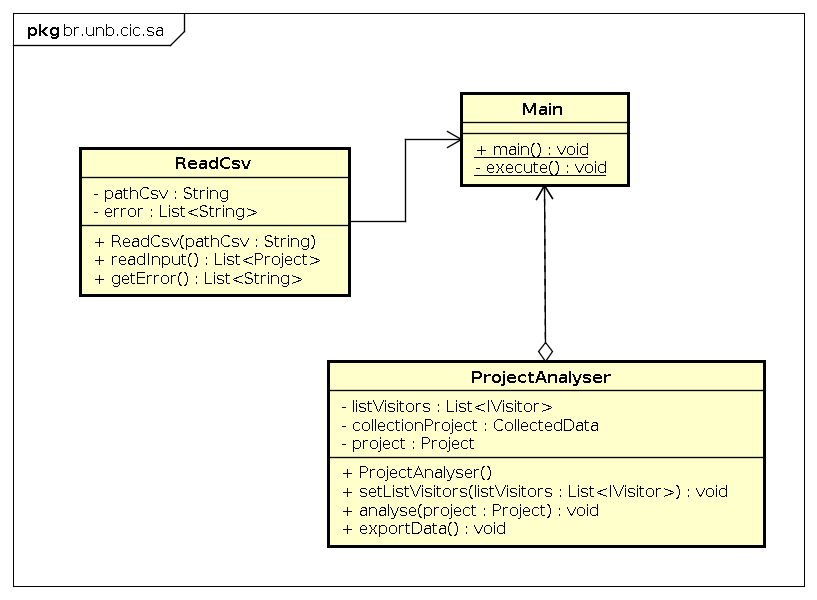
\includegraphics[scale=0.55]{Imagens/Arquitetura}
	\label{fig:Arquitetura}
	\caption{Alto nível de funcionamento do analisador estático.}
\end{figure}

 No mais elevado nível de abstração do analisador estático a Figura:~\ref{fig:Arquitetura} demonstra seu funcionamento que é encontrar um código fonte Java, criar um \textit{Parse} que é uma representação intermediária deste código fonte em seguida é aplicado uma série de mecanismos de análise estática para coletar as informações de interesse no código fonte e por fim é gerado relatórios~\acs{CSV}.

Atualmente existem diversas tecnologias capazes de prover ferramentas para implementar um analisador estático entretanto devido a maior experiência com uso da linguagem Java, neste projeto foi utilizado a infraestrutura da plataforma Eclipse JDT, \textit{Eclipse Java Development Tools}~\cite{EclipseJDT}. O EclipseJDT~\cite{EclipseJDT} fornece um conjunto de ferramentas que contribuem com elaboração uma análise sobre o código Java.

A biblioteca JDT é composta 4 componentes \textit{APT, Core, Debug} e \textit{UI}, neste projeto a adoção deu-se através do \textit{JDT Core} que dispõe de uma modelo Java para a navegação dos elementos de uma árvore sintática,~\acs{AST}, onde os elementos podem ser pacotes, tipos, métodos e atributos. Também existe API pronta para a manipulação de código fonte.

A~\acs{AST} provida pelo JDT é composta por 122 classes, como por exemplo existem 22 classe para representar palavras reservadas \textit{IF-Than-Else, Switch, While, BreakStatement} e outras. Exitem 5 classes que trabalham exclusivamente com métodos referenciados, e 6 classes exclusiva que tratam somente os tipos declarados em um classe Java.

O Eclipse JDT~\cite{EclipseJDT} fornece para este projeto um \textit{Parser} que produz uma representação intermediária baseada em um conjunto de classes Java que representam uma ~\acs{AST} de um código fonte. Fornece ainda uma infraestrutura de \textit{visitors}~\cite{Gamma:1995} que possibilitam a análise estática de código fonte.

Um \textit{visitor} é um padrão de projetos proposto por Eric Gamma~\cite{Gamma:1995}, este padrão de projeto de característica comportamental que representa uma operação a ser realizada sobre elementos de uma estrutura de um objetos. Neste caso operação a ser realizadas é visitar os nós de uma árvore sintática de um código fonte Java. Um \textit{visitor} permite que uma nova operação seja criada sem que os elementos operados sofram alterações. Com isso é trivial adicionar novas funcionalidades em um \textit{visitor} existente ou criar um novo.

A biblioteca Eclipse JDT não fornece mecanismo para extração de dados, entretanto foi acoplado um conjunto de classe visando obter a maior facilidade e flexibilidade na geração dos relatórios com os dados contidos na análise estática realizada. Essa flexibilidade foi alcançada com a utilização de introspecção de código que em Java é conhecido como \textit{reflection}.


\section{Entrada de dados}

\begin{figure}[h]
	\center
	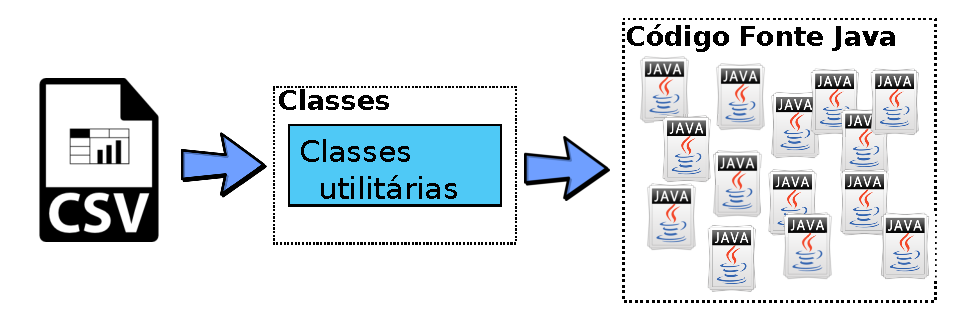
\includegraphics[scale=0.55]{Imagens/InputArquitetura}
	\label{fig:InputArquitetura}
	\caption{Input para funcionamento do analisador estático.}
\end{figure}

A entrada do analisador estático é iniciado com um arquivo \acs{CSV} que contém nome dos projetos, caminho e quantidade de linhas de código conforme demonstrado na Figura:~\ref{fig:InputArquitetura}. As informações contidas no arquivo \acs{CSV} são extraídas por um conjunto de classes utilitárias que varrem os diretórios de um determinado projeto pesquisando por todos os arquivos fonte Java. Os códigos fontes Java encontrados são a entrada descrita no funcionamento em alto nível da Figura:~\ref{fig:Arquitetura}. Onde para cada projeto é feito a varredura de arquivos Java, gerado o \textit{Parser} dos códigos Java e exportar os relatórios.

\section{Análise Estática}

\begin{figure}[h]
	\center
	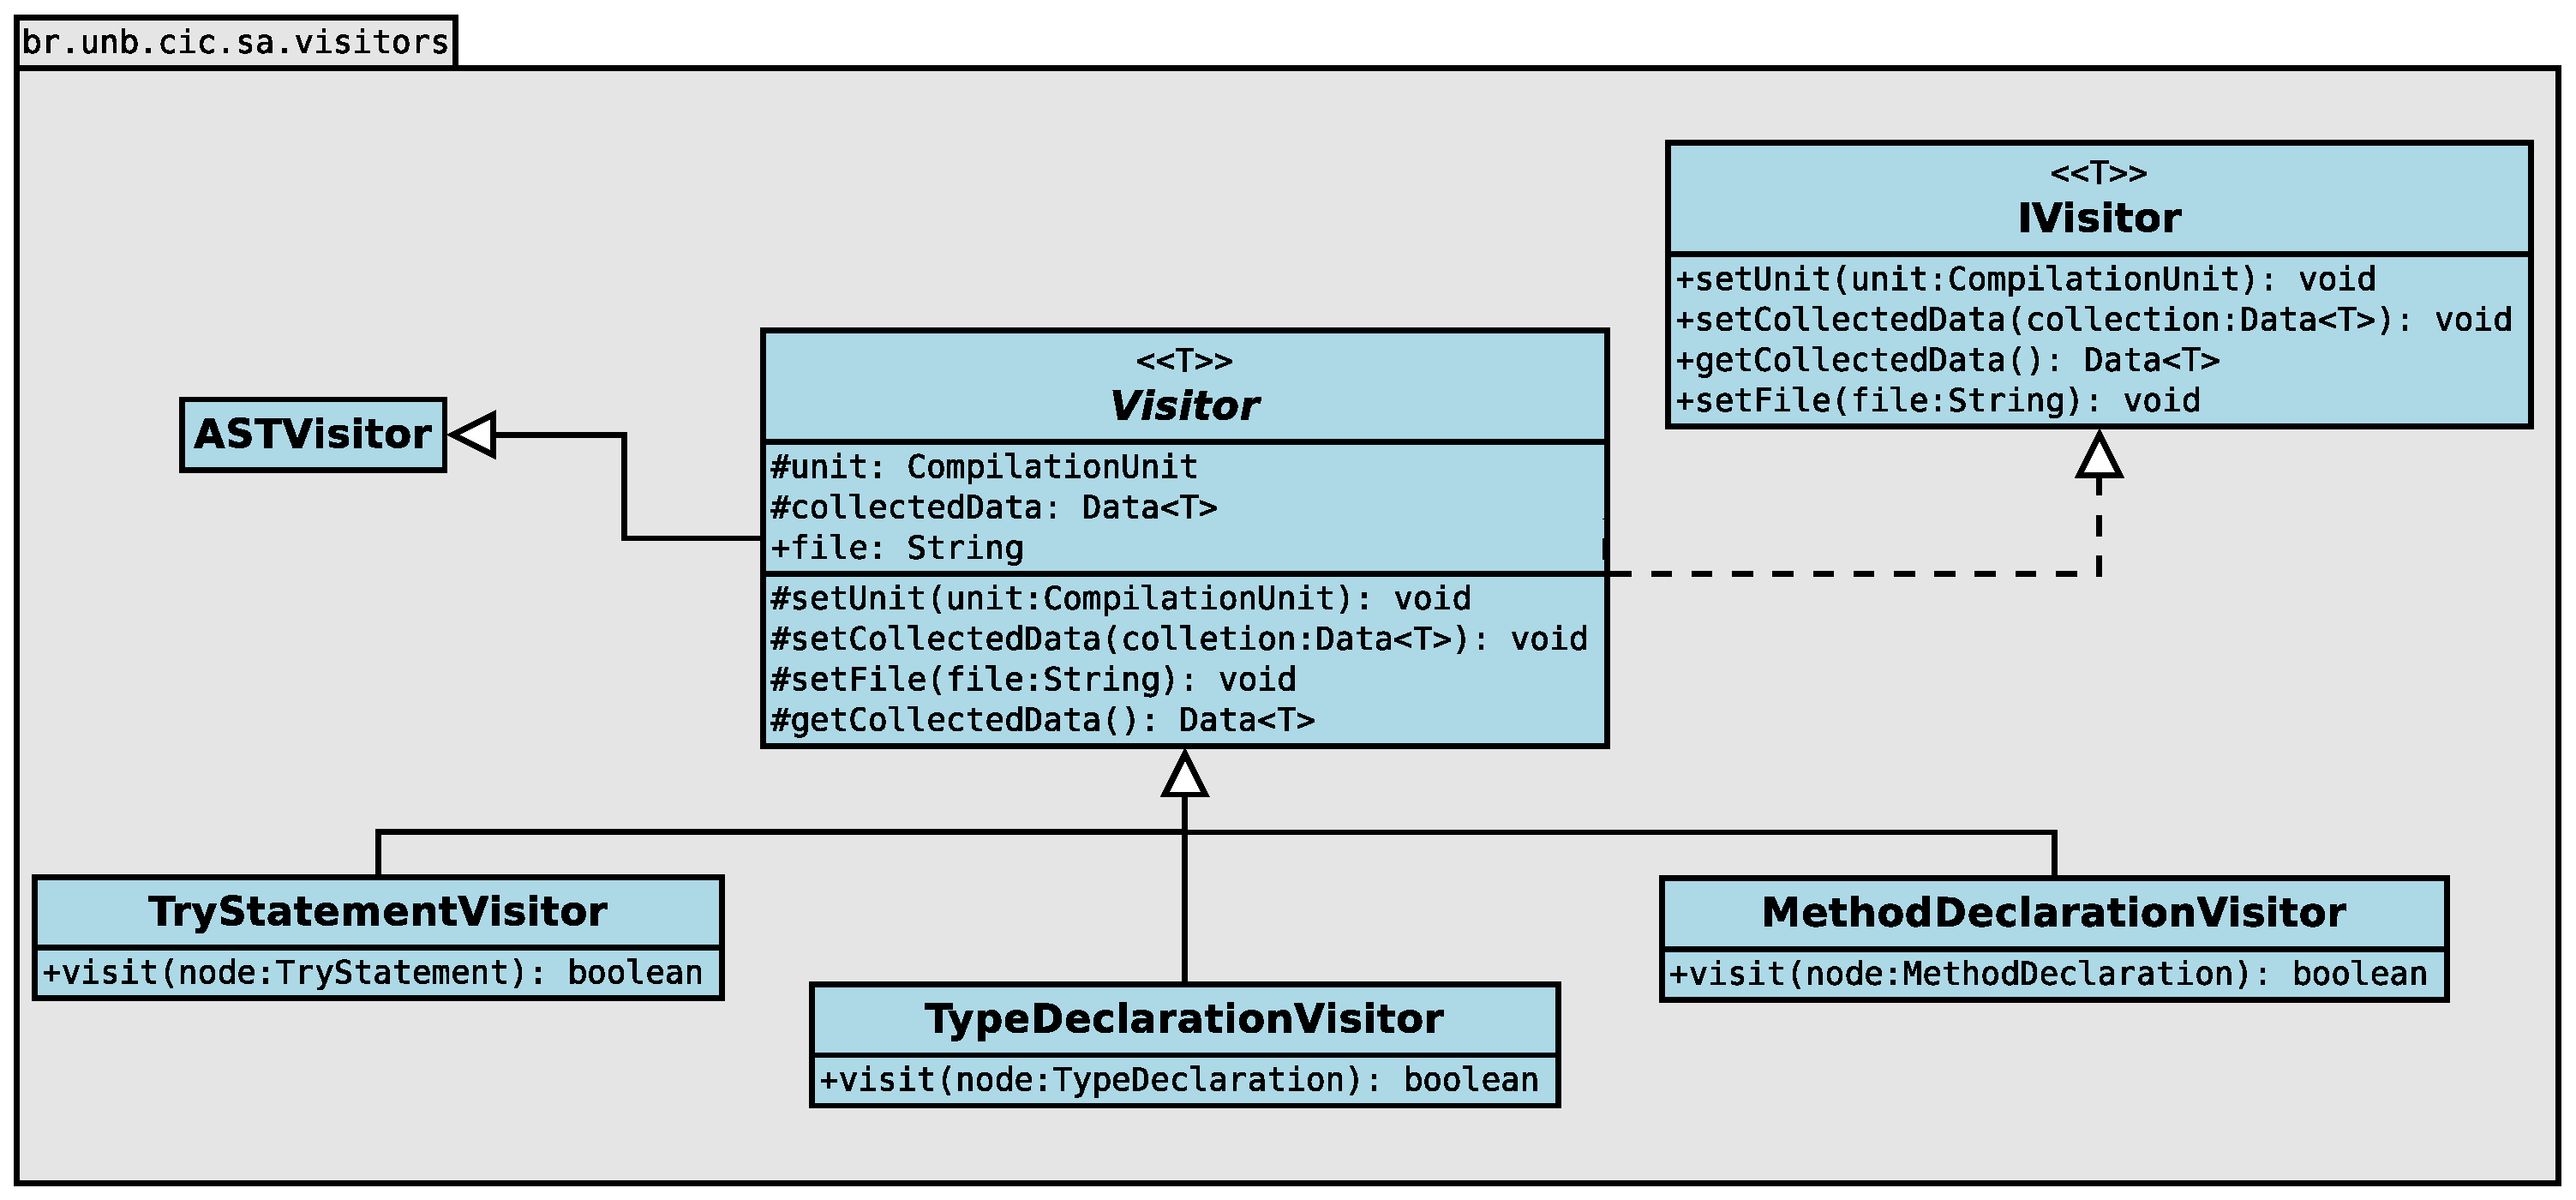
\includegraphics[scale=0.25]{Imagens/diagramaVisitor}
	\label{fig:DiagramaVisitor}
	\caption{Diagrama Visitor.}
\end{figure}

Após o \textit{Parser} é feita a coleta de dados utilizando uma infraestrutura de \textit{Visitors}. Onde para este projeto uma classe \textit{Visitor} é parametrizada em um tipo \textbf{T}, \textbf{\textit{Visitor<T>}}, onde este tipo \textbf{T} é a classe criada que vai armazenar as informações coletadas, conforme o diagrama da Figura:~\ref{fig:DiagramaVisitor}. O parâmetro \textbf{<T>} descrito faz referência a uma classe modelo composta por \textit{getters} e \textit{setters} para modelar os dados extraídos e que sejam armazenados corretamente. 

Confome exemplificado na Figura:~\ref*{fig:DiagramaVisitor}, com a necessidade de criar um \textit{Visitor} que detecte e colete informações dos tipos declarados no sistema, basta criar uma classes modelo \textit{TypeDeclaration.java} e  setar o parâmetro \textbf{<T>} como \textit{<TypeDeclaration>}, com isso os dados serão extraídas pelo \textit{Visitor, TypeDeclarationVisitor.java}, que identifica as informações pertinentes. 

A Tabela:~\ref{tab:VisitorsCriados} exibe todos os \textit{Visitors} criados neste projeto com sua respectiva descrição.

\begin{table}[ht!] \footnotesize
	\centering
	\caption{Tabela de Visitors criados com suas respectivas atribuições}
	\label{tab:VisitorsCriados}	
    \begin{tabular}{ >{\arraybackslash}p{2.5in} | >{\arraybackslash}m{3.5in} }
%		\begin{tabular}{M|p{9cm}}% centered column
			\hline 
			\textbf{Visitor} & \textbf{Atribuição}\\ \hline \hline
			
			AICVisitor & Pesquisar \textit{Anonymous Inner Class} declaradas.\\ \hline
			
			EnumDeclarationVisitor 	& Pesquisa por \textit{Enums} declarados.\\ \hline
			
			ExistPatternVisitor	& Pesquisa \textit{EnhancedFor} que iteram sobre uma coleção procurando qualquer ocorrência nessa coleção.\\ \hline
			
			FieldAndVariableDeclarationVisitor & Lista todos as variáveis declaradas como os respectivos tipos.\\ \hline
			
			FilterPatternVisitor &  Lista todos os \textit{EnhancedFor} que iteram uma coleção filtrando elementos desta mesma coleção.\\ \hline
			
			ImportDeclarationVisitor & Lista todos os \textit{imports}.\\ \hline
			
			LambdaExpressionVisitor & Pesquisa casos de utilização da expressões lambda. \\ \hline
			
			LockVisitor & Verifica se nos métodos declarados existe alguma variável chamada Lock, ReentrantLock, ReadLock ou WriteLock. \\ \hline
			
			MapPatternVisitor & Pesquisa \textit{EnhancedFor} que iteram sobre uma coleção onde seja aplicado algum método sobre os itens desta coleção. \\ \hline
			
			MethodCallVisitor & Verifica onde esta sendo utilizado reflection no projeto.\\ \hline
			
			MethodDeclarationVisitor & Coleta informações sobre os métodos declarados nos projetos. \\ \hline
			
			ScriptingEngineVisitor & Verifica se o projeto faz chamada a algum \textit{Scripting}.\\ \hline
			
			SwitchStatementVisitor & Pesquisa \textit{Switchs} que utilizam \textit{String} como parâmetro.\\ \hline
			
			SwitchStringOpportunitiesVisitor &  Pesquisa \textit{If-Else} aninhados onde no \textit{If} contenha \textit{String}, caracterizando uma possibilidade de adoção de \textit{Switch} com \textit{String}.\\ \hline
		
			TryStatementVisitor & Pesquisa \textit{trys} que utilizar \textit{resource}, adoção de \textit{multicatch} e \textit{trys} que possuem \textit{catchs} aninhados.\\ \hline
			
			TypeDeclarationVisitor & Pesquisa todos os tipos declarados.\\ \hline 		
		\end{tabular}
\end{table}

\section{Extensibilidade da Plataforma}

\subsection{Injeçao de Dependência}
Injeção de dependência \acs{DI}, originalmente foi denominado inversão de controle \acs{IoC} pois a sequência de criação dos objetos depende de como são solicitados pelo sistema. Quando um sistema é iniciado todos os objetos que o compoe são criados mas utilizando. Entretanto isto não acontece quando é utilizado \acs{DI} pois os objetos serão criados, injetados, a medida que são necessitados pelo sistema.

A extensibilidade da plataforma é alcançada devido o conceito de \acs{DI} através do \textit{framework} Spring~\cite{SPRING_REF} para flexibilixar a criação de \textit{Visitors}. Com isso o acoplamento entre a classe que cria a árvore sintática de um código fonte e a classe que analisa esta árvore possuem um baixo acoplamento pois quando for solicitado um \textit{visitor} para uma pesquisa o \textit{framework} Spring~\cite{SPRING_REF} saberá o momento certo de instanciar e injetar o \textit{visitor} na classe que o solicita.

Devido este conceito adotado no sistema o desenvolvedor deve concentrar seu esforço na criação de \textit{visitors} fazendo como que estes extraim as informações mais precisas bastando somente declarar o \textit{visitor} criado no arquivo \textit{bean.xml} do Spring~\cite{SPRING_REF}.

\subsection{Reflection}
Também focando na flexibilidade do sistema, a geração de relatórios é dada baseado no conceito de \textit{Reflection} que é a introspecção de código que Java possui. Isto é a capacidade de um programa possui de se observar e até modificar sua estrutura ou comportamento em tempo de execução.

\begin{figure}[h]
	\center
	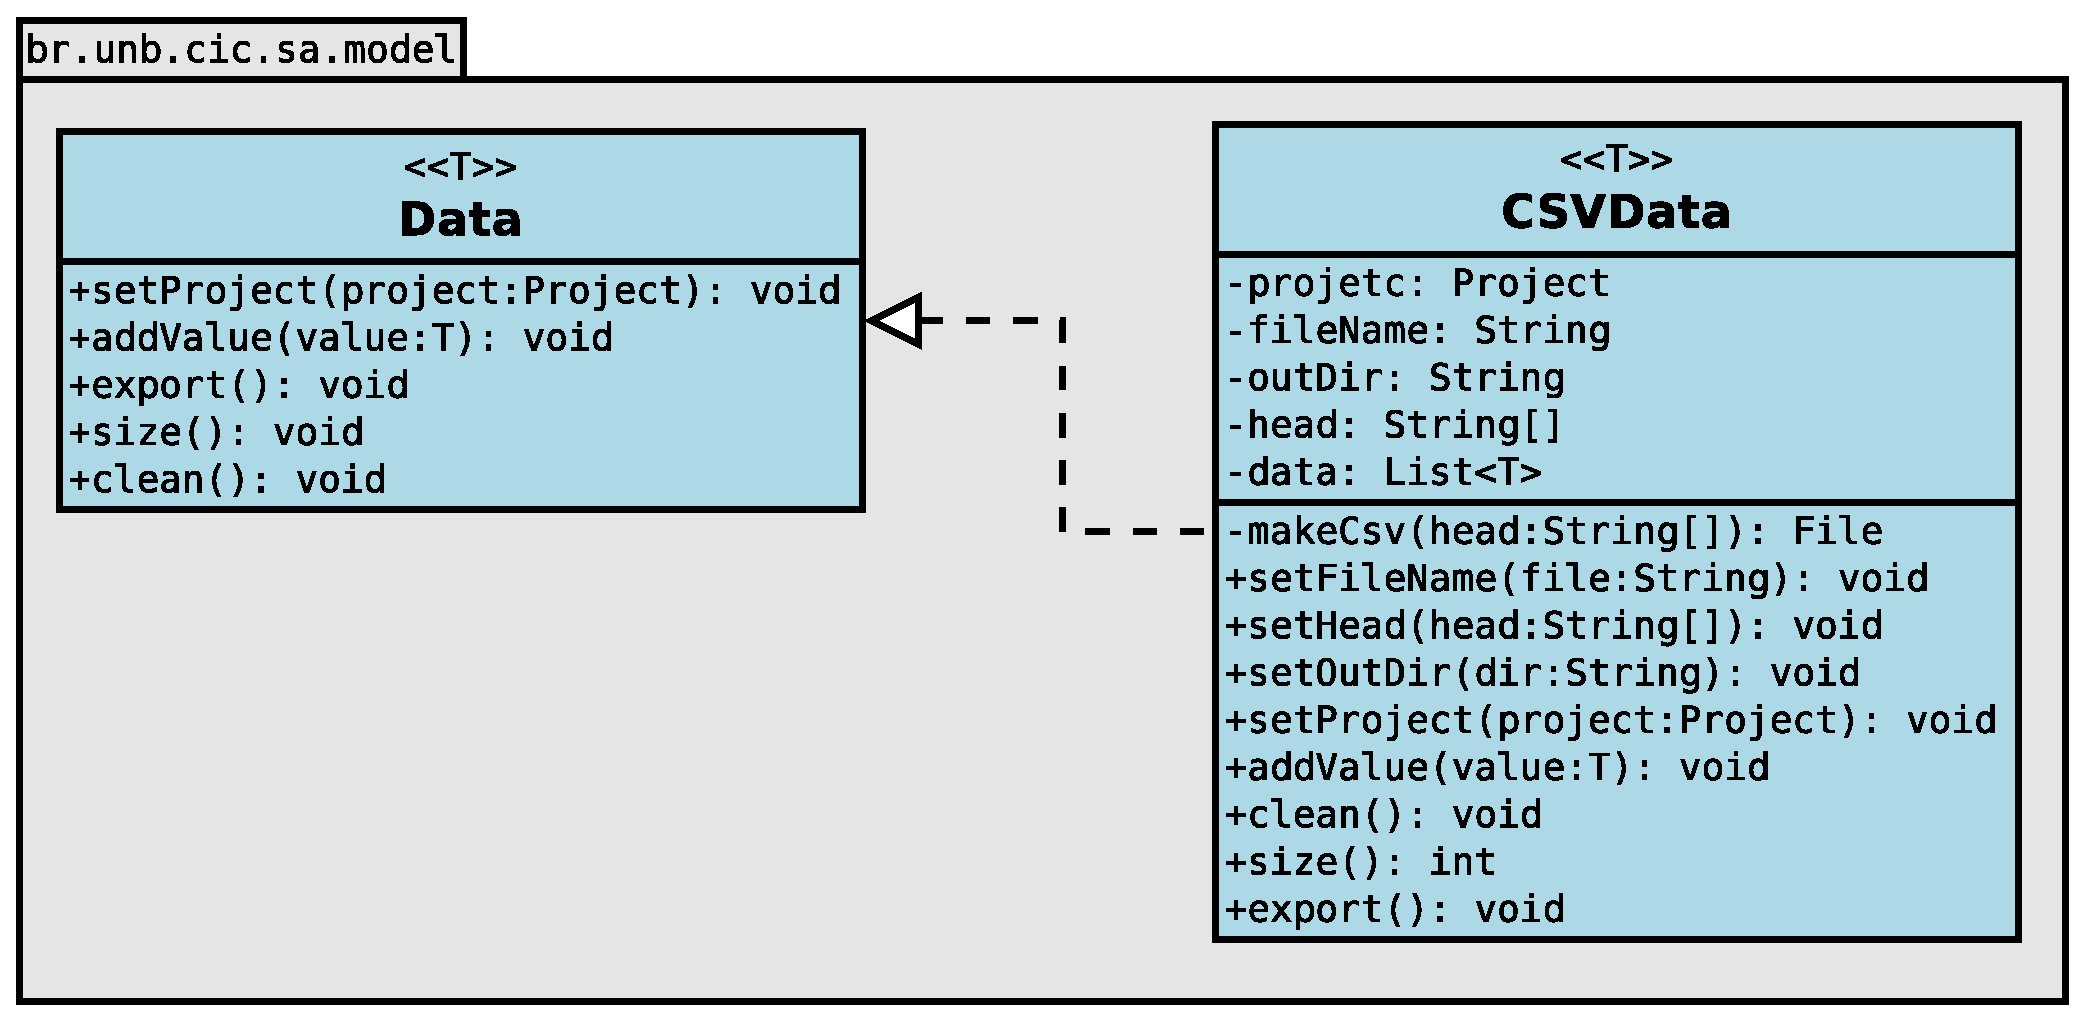
\includegraphics[scale=0.35]{Imagens/diagramaCSVData}
	\label{fig:DiagramaCSVData}
	\caption{Diagrama geração de relatórios.}
\end{figure}

A geração dos relatórios ocorre utilizando a classe \textbf{CSVData<T>} onde o tipo \textbf{<T>} é o mesmo utilizado modelar os dados coletados pelos \textit{Visitors}. Os dados são obtidos através dos métodos \textit{getters} destas classes modelos e exportados para arquivos ~\acs{CSV}, nesta classe também existe a injeção de dependência que é somente o cabeçalho do arquivo ~\acs{CSV} o qual é declarado no \textit{beans.xml} ao mesmo tempo em que o \textit{Visitor} é declarado, a Figura:~\ref{fig:DiagramaCSVData} exibe o diagrama de classe.

O cabeçalho de cada \acs{CSV} é injetado pelo Spring no atributo \textbf{head:String[]}. Logo em seguida o método \textit{export()} da classe \textbf{CSVData<T>} inicia seu trabalho realizando introspecção recuperando de uma coleção dos dados armazenados do projeto, lista \textbf{Data<T>}. Após a recuperação destes dados é realizada o \textit{reflection} para recuperar cada classe modelo e com isso detectar todos os métodos \textit{getters} destas classes e como isso imprimir-los no relatório que é o arquivo \acs{CSV} de saída. 

\begin{lstlisting}

public class CSVData<T> implements Data<T>{
	...
	@Override
	public void export() {
		try (FileWriter writer = 
			new FileWriter(this.makeCsv(head), true)){
		
			StringBuffer str = new StringBuffer("");

			if(data == null) { return;	}
			
			for(T value : data) {
				//reflection code...
				for(Field f: value.getClass().getDeclaredFields()){
										
					String fieldName = f.getName();
					String prefix = "get";
					
					if(f.getType().isPrimitive() &&
						f.getType().equals(Boolean.TYPE)) {
						prefix = "is";
					}
					
					String methodName = prefix +
					 	Character.toUpperCase(fieldName.charAt(0)) +
					 	fieldName.substring(1);
										
					try {
						Method m = value.getClass().getDeclaredMethod(methodName);						
						str.append(m.invoke(value));
						str.append(";");
					}catch(NoSuchMethodException |  IllegalAccessException | 
						   IllegalArgumentException | InvocationTargetException e) {
						throw new RuntimeException("Type " + 
											value.getClass().getName() +
											" must have a method named " + methodName);
					}
				}
				writer.append(str.toString());
				writer.append("\n");
				
			}
			writer.flush();

		}catch(Exception e) {
			e.printStackTrace();
		}
	}
}
\end{lstlisting}


%Projetar um analisador estático para extrair informações de softwares desenvolvido não é uma simples tarefa, entretanto EclipseJDT~\cite{EclipseJDT} prove uma abstração significativa tornado menos árdua este projeto. O que pode possibilitar projetar uma arquitetura mais robusta para este analisador onde o foco de qualquer desenvolvedor que deseje utilizá-lo concentre-se apenas na produção de seus \textit{Visitors}. 
%
%Um ponto de extrema relevância foi tornar este analisador independente de qualquer plataforma e \acs{IDE} foi um ponto vital para o concepção deste projeto que não tem como intuito ser plugin de qualquer \acs{IDE} o que acarretaria na limitação do seu uso a um cenário específico mas sim uma ferramenta para apoiar no desenvolvimento de um software com construções atuais. Utilizando a portabilidade nativa entre as plataformas provido pela linguagem Java este trabalho foi concebido com intuito de atender ao mais diversos desenvolvedores quer utilizem Linux, Windows, Mac ou qualquer outro sistema operacional que tenha suporte para Java.
%
%A análise tem como início a seleção de projetos, nesse caso seleção em repositórios públicos, onde após o download é informado analisador o diretório raiz onde estes estão localizados. Após é iniciado uma listagem dos arquivos fonte Java contidos nos projeto e contabilizados o total de \acs{LOC} e criado uma árvore sintática para cada arquivo encontrado através de um \textit{parser} provido pela biblioteca EclipseJDT~\cite{EclipseJDT}. Em seguida os \textit{Visitors} são instanciados com o objetivo de percorrer os nós destas árvores para pesquisar por construções de código previamente determinadas.
%
%Todas as construções pesquisadas quando encontradas pelos \textit{Visitors} são armazenadas temporariamente enquanto o analisador verifica todo projeto, quando é verificado a última árvore sintática pelos \textit{Visitors} é iniciado o processo de exportar os dados encontrados para um arquivo \acs{CSV} o conteúdo relevante destes blocos, a Figura:~\ref{fig:Arquitetura} demostra de maneira clara o funcionamento do analisador. Após a exportação dos dados o analisador inicia todo processo novamente caso exista mais de um projeto.
%
%Devido ao mecanismo de \textit{reflection} proveniente da linguagem Java, o desenvolvedor não tem a necessidade de implementar código para exportação de dados tendo em vista que isto ocorre automaticamente através da introspecção realizada pelo analisador extraindo os dados armazenados pelos \textit{Visitors}.

%	\begin{figure}[h]
%		\center
%		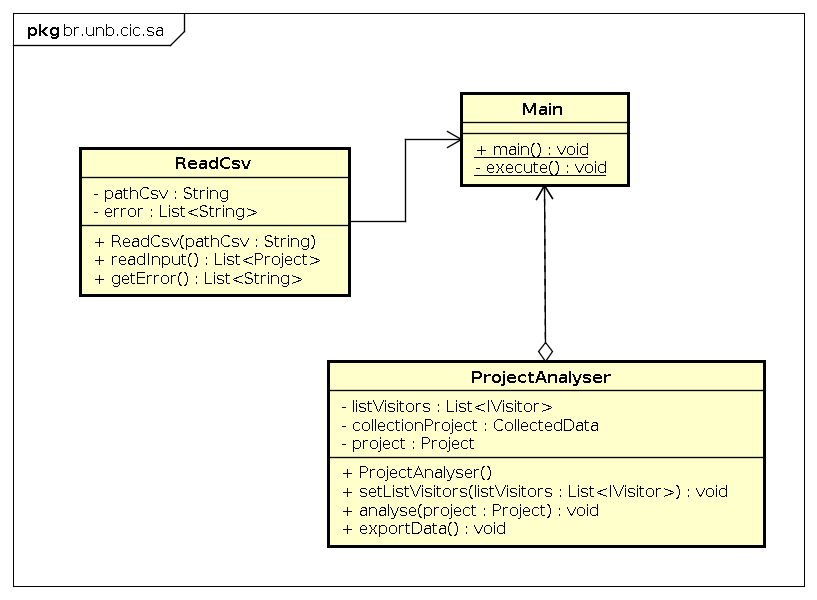
\includegraphics[scale=0.52]{Imagens/Arquitetura}
%		\label{fig:Arquitetura}
%		\caption{Funcionamento analisador estático.}
%	\end{figure}


%\section{Arquitetura}
%
%\subsection{Visitors}
%
%
%
%\begin{lstlisting}
%package br.unb.cic.sa.visitors;
%
%import org.eclipse.jdt.core.dom.ASTVisitor;
%import org.eclipse.jdt.core.dom.CompilationUnit;
%import br.unb.cic.sa.model.Data;
%
%public class Visitor<T> extends ASTVisitor implements IVisitor<T> {
%	protected CompilationUnit unit;
%	protected Data<T> collectedData;
%	protected String file;
%	
%	public Visitor() {}
%	
%	@Override
%	public void setUnit(CompilationUnit unit) { this.unit = unit; }
%	
%	@Override
%	public void setCollectedData(Data<T> colletion) { this.collectedData = colletion; }
%	
%	@Override
%	public void setFile(String file) {	this.file = file; }
%
%	@Override
%	public Data<T> getCollectedData() {	return collectedData;	}	
%}
%\end{lstlisting}
%
%
%A tabela:~\ref{tab:VisitorsCriados} detalha os 17 \textit{Visitors} criados com a respectiva descrição do trabalho realizado. Como forma de exemplificar a criação de um \textit{Visitors}, etapa a qual é composta de 4 passos quo serão demonstrados a seguir.
%
%A investigação para saber como o tratamento de exceção Java tem sido utilizado acarretou na criação de um \textit{Visitor} específico para este fim, \textit{TryStatementVisitor}, responsável por pesquisar este mecanismo o qual pode contar com alguma evoluções ao logo do histórico da linguagem Java. A pesquisa é iniciada encontrando blocos \textit{trys/catch}, onde destes será coletadas as informações referentes a adoção de \textit{resources} e oportunidade de utilizar \textit{multicatch} em blocos \textit{trys} que contenham \textit{catchs} iguais aninhados.
%%, neste caso de oportunidades os \textit{catchs} são testados por igualdade mas é trivial a utilização de um algoritmo mais avançado que teste a similaridade.
%
%Criação do \textit{Visitor TryStatementVisitor} com exemplo.
%
%	\begin{enumerate}
%		\item Inicialmente é necessário criar a classe modelo onde esta terá atribuição de receber os dados que serão extraídos pelos \textit{Visitors}, basicamente as classes modelos são compostas de \textit{getters} e \textit{setters} e são declaradas no pacote  \textit{\textbf{br.unb.cic.sa.model}}.
%			\begin{lstlisting}
%package br.unb.cic.sa.model;
%
%public class TryStatementData  {
%	private String file;
%	private int startLine;
%	private int endLine;
%	private boolean tryWithResource = false;
%	private boolean multiCatch = false;
%	
%	public TryStatementData(String file, int startLine, int endLine){
%		this.file = file;
%		this.startLine = startLine;
%		this.endLine = endLine;
%	}
%	
%	//getters and setters
%}
%			\end{lstlisting}
%			
%			
%		\item Em seguida, é concebida a criação do \textit{Visitor} no pacote \textit{\textbf{br.unb.cic.sa.visitors}} onde esta nova classe será estendida da classe parametrizada \textit{\textbf{Visitor<TryStatementData>}} apresentada anteriormente onde a parametrização desta classe é o modelo criado anteriormente.
%			
%			\begin{lstlisting}
%package br.unb.cic.sa.visitors;
%
%import java.util.List;
%import org.eclipse.jdt.core.dom.CatchClause;
%import org.eclipse.jdt.core.dom.TryStatement;
%import br.unb.cic.sa.model.TryStatementData;
%import br.unb.cic.sa.similarity.BasicSimilarityChecker;
%import br.unb.cic.sa.similarity.SimilarityChecker;
%
%public class TryStatementVisitor extends Visitor<TryStatementData> {
%
%	SimilarityChecker similarity;
%
%	public TryStatementVisitor() {
%		similarity = new BasicSimilarityChecker();
%	}
%
%	@Override
%	public boolean visit(s node) {
%
%		TryStatementData t = new TryStatementData(this.file, unit.getLineNumber(node.getStartPosition()),
%				unit.getLineNumber(node.getStartPosition() + node.getLength()));
%		
%		if (node.resources().size() > 0) {
%			t.setTryWithResource(true);
%		}
%	
%		if (node.catchClauses().size() > 1) {
%			if (this.checkSimilarity(node.catchClauses())) {
%				t.setMultiCatch(true);
%			}
%		}
%
%		this.collectedData.addValue(t);
%
%		return super.visit(node);
%	}
%	
%	private boolean checkSimilarity(List<CatchClause> catchClause) {
%		for (CatchClause cc : catchClause) {
%			for (CatchClause cn : catchClause) {
%				// To ignore the same catch in loops
%				if (!cc.equals(cn)) {
%				
%				//Chamada externa para testar similaridade
%					if (this.similarity.checkSimilarity(cc.getBody(),
%														cn.getBody())) {
%						return true;
%					}
%				}
%			}
%		}
%		return false;
%	}
%
%}
%			\end{lstlisting}
%			
%		 Na linha24, é testada a condição para saber se este bloco fez adoção de \textit{Resouce}. Na linha 30 é verificado que o bloco é um possível caso de \textit{multicatch} pois existe mais de um bloco. Na linha 39 tem-se o método \textit{checkSimilarity} o qual efetua a comparação dos blocos \textit{Catch} aninhados, entretando de forma trivial na linha 46, pode ser utilizado um algoritmo mais sofisticado para testar por similaridade modificando apenas o conteúdo do método \textbf{\textit{checkSimilarity}} da classe \textit{\textbf{SimilarityChecker}} o que não resulta em mudanças neste \textit{Visitor}.
%		
%	
%			\item Em seguida deve-se declarar o cabeçalho no arquivo \textit{resource/Beans.xml} do \textit{Spring} que estará presente no \acs{CSV} de saída. Onde este cabeçalho é composto pelo dados que serão extraídos pelos \textit{Visitors} e armazenados no modelo criado.
%			
%			\begin{lstlisting}
%<bean id="tryStatementData" class="br.unb.cic.sa.model.CSVData">
%	<property name="outDir" value="output"/>
%	<property name="fileName" value="tryStatement"/>
%	<property name="head" value="typeProject, before, project, version, file, start, end, resource, multiCatch"/> 
%</bean>
%			\end{lstlisting}
%			
%			
%			\item Por fim declarar o \textit{Visitor} como um \textit{bean} do \textit{Spring} para que este seja injetado no projeto e assim realize sua pesquisa.
%			
%			\begin{lstlisting}
%<bean id="tryStatementVisitor" class="br.unb.cic.sa.visitors.TryStatementVisitor">
%	<property name="collectedData" ref="tryStatementData"/>
%</bean>
%			\end{lstlisting}
%			
%	\end{enumerate}
%
%
%
%\subsection{Exportar Dados}
%A exportação dos dados para \acs{CSV} é realizado de forma automática utilizando o mecanismo de \textit{reflection} fornecido por Java. A classe parametrizada \textbf{\textit{CSVData<T>}} no pacote \textbf{\textit{br.unb.cic.sa.model}} implementa a interface \textit{\textbf{Data<T>}} onde \textbf{\textit{<T>}} faz  aos modelos declarados para as informações coletadas.
%
%\begin{lstlisting}
%package br.unb.cic.sa.model;
%
%public interface Data<T> {
%	public void setProject(Project project);
%	public void addValue(T value);
%	public void export();
%	public int size();
%	public void clean();
%}
%\end{lstlisting}
%
%
%Onde o atributo \textit{String[] head} é injetado pelo \textit{Spring} pois fora declarado anteriormente na criação do visitor. O método \textbf\textit{{export()}}, na linha 23, é o método responsável para exportar os dados em seus respectivos \acs{CSV} pois este método recupera as informações contidas nas coleções populadas pelos \textit{Visitors} e com \textit{reflection} captura os campos declarados em especial para os métodos quais são pré-fixados com \textit{get ou is} que terão seus valores capturados para que sejam exportados.
%
%\begin{lstlisting}
%package br.unb.cic.sa.model;
%
%import java.io.File;
%import java.io.FileWriter;
%import java.io.IOException;
%import java.lang.reflect.Field;
%import java.lang.reflect.InvocationTargetException;
%import java.lang.reflect.Method;
%import java.util.ArrayList;
%import java.util.List;
%
%public class CSVData<T> implements Data<T>{
%
%	private Project project;
%	private String fileName;
%	private String outDir;
%	private String[] head; 
%	private List<T> data;
%
%	...
%	
%	@Override
%	public void export() {
%		
%		try (FileWriter writer = new FileWriter(this.makeCsv(head), true)){
%		
%			StringBuffer str = new StringBuffer("");
%
%			if(data == null) {
%				return;
%			}
%			
%			for(T value : data) {
%				str = new StringBuffer("");
%				
%				str.append(project.getTypeOfProject());
%				str.append(";");
%				str.append(project.getBefore());
%				str.append(";");
%				str.append(project.getProjectName());
%				str.append(";");
%				str.append(project.getProjectRevision());
%				str.append(";");
%			
%				for(Field f: value.getClass().getDeclaredFields()){
%										
%					String fieldName = f.getName();
%					String prefix = "get";
%					
%					if(f.getType().isPrimitive() &&
%					   f.getType().equals(Boolean.TYPE)) {
%						prefix = "is";
%					}
%					
%					String methodName = prefix + 
%								Character.toUpperCase(fieldName.charAt(0)) +
%								fieldName.substring(1);
%										
%					try {
%						Method m = value.getClass().getDeclaredMethod(methodName);						
%						str.append(m.invoke(value));
%						str.append(";");
%					}catch(
%							NoSuchMethodException | 
%							IllegalAccessException |
%							IllegalArgumentException |
%							InvocationTargetException e) {
%							
%						throw new RuntimeException("Type " + 
%											value.getClass().getName() +
%											" must have a method named " +
%											 methodName);
%					}
%				}
%				
%				writer.append(str.toString());
%				writer.append("\n");
%				
%			}
%		
%			writer.flush();
%		
%		}
%		catch(Exception e) {
%			e.printStackTrace();
%		}
%	}
%}
%
%\end{lstlisting}